\documentclass[a4paper,11pt, hidelinks]{article}

\usepackage{listings}
\usepackage{lmodern}
\usepackage{amsmath,amssymb,amsthm,textcomp}
\usepackage[utf8]{inputenc}  
\usepackage[T1]{fontenc}  
\usepackage{graphicx}
\usepackage{float}
\usepackage{enumitem}
\usepackage{bbm}
\usepackage{caption}
\usepackage{hyperref}
\usepackage{cancel}
\usepackage{bigints}
\graphicspath{ {images/} }

\usepackage{geometry}
\geometry{total={210mm,297mm},
left=15mm,right=15mm,%
bindingoffset=0mm, top=30mm,bottom=30mm}

\usepackage{etoolbox}
\makeatletter
\preto{\@verbatim}{\topsep=0pt \partopsep=3pt }
\makeatother

\linespread{1}

\newcommand{\linia}{\rule{\linewidth}{0.5pt}}


% my own titles
\makeatletter
\renewcommand{\maketitle}{
\begin{center}
\vspace{2ex}
{\huge \textsc{\@title}}
\vspace{1ex}
\\
\linia\\
\@author 
\vspace{4ex}
\end{center}
}
\makeatother
%%%

% custom footers and headers
\usepackage{fancyhdr}
\pagestyle{fancy}
\lhead{}
\chead{}
\rhead{}

\cfoot{}
\rfoot{Page \thepage}
\renewcommand{\headrulewidth}{0pt}
\renewcommand{\footrulewidth}{0pt}
%
\DeclareMathOperator*{\argmax}{arg\,max}
\DeclareMathOperator*{\argmin}{arg\,min}
\DeclareMathOperator*{\var}{var}
\DeclareMathOperator*{\cov}{cov}
\DeclareMathOperator*{\tr}{tr}

%%%----------%%%----------%%%----------%%%----------%%%

\begin{document}

\title{HW2}

\author{Gabriel ROMON}



\maketitle

\section*{2 Multilingual word embeddings}

Remember that the Frobenius norm on $\mathbb R^{d,m}$ is induced by the inner product $\langle A,B \rangle_F = \tr(A^TB)$. Consequently $$\|WX - Y\|_F^2 = \|WX\|_F^2 + \|Y\|_F^2 - 2\langle WX, Y\rangle_F$$
Since $W$ is orthogonal, $\|WX\|_F^2 = \tr(X^TW^TWX) = \tr(X^TX) = \|X\|_F^2$ and by the cyclic property of trace $\langle WX, Y\rangle_F = \tr(X^TW^TY) = \tr(W^TYX^T) = \langle W, YX^T\rangle_F$, hence 
$$\|WX - Y\|_F^2 = \|X\|_F^2 + \|Y\|_F^2  -2\langle W, YX^T\rangle_F $$ We may therefore look for $\argmax_{W\in O_d(\mathbb R)} \langle W, YX^T\rangle_F$.\newline
Let $U, V\in O_d(\mathbb R)$ and $\Sigma \in \mathbb R^{d,d}$ a diagonal matrix with positive entries such that $YX^T = U\Sigma V^T$. From the cyclic property of trace, $$\langle W,U\Sigma V^T\rangle_F = \langle U^TW V,\Sigma\rangle_F$$
Note that $Z:=U^TW V$ is orthogonal as a product of orthogonal matrices and $\langle Z,\Sigma\rangle_F = \sum_{i=1}^d \Sigma_{ii} Z_{ii}$. Since $Z$ is orthogonal its entries are $\leq 1$ in absolute value and since the singular values $\Sigma_{ii}$ are $>0$ we infer that $\langle Z,\Sigma\rangle_F \leq \sum_{i=1}^d \Sigma_{ii}$ with equality when $Z=I_d$, which yields the optimal $W$ as $UV^T$.


\section*{3 Sentence classification with BoV}

We tune the value of the regularization parameter on the dev set, with and without IDF weighting. The accuracies of the corresponding best models are reported in Figure 1.
\begin{figure}[H]
\centering
\begin{tabular}{|c|c|c|} \hline
 &  Average & IDF-weighted average \\ \hline
\begin{tabular}{c} Train set
\end{tabular} &
\begin{tabular}{c} 48.68\%
\end{tabular} &
\begin{tabular}{c} 48.85\%
\end{tabular}  \\ \hline
\begin{tabular}{c} Dev set
\end{tabular} &
\begin{tabular}{c} 43.05\%
\end{tabular} &
\begin{tabular}{c} 41.78\%
\end{tabular}  \\ \hline
\end{tabular}
\captionof{table}{Accuracy of the best model}
\end{figure}


\section*{4 Deep Learning models for classification}

\begin{enumerate}[label=(\alph*)]
\item The loss that yielded the best results is the categorical cross-entropy. For a single data point $x$ with true label $k$ it is equal to $-\log p$ where $p$ is the predicted probability that $x$ belongs to class $k$. It may also be written as $$-\sum_{i=0}^4 1_{c(x)=k} \log(p_k)$$ where $(p_0,\ldots,p_4)$ is the vector of probabilities returned by the model for the instance $x$.

\item I chose not to use IDF weighting. The accuracies on the train and dev set for each epoch are reported in Figure 1. Since there is not so much data very few epochs (around 4) are sufficient to reach convergence.
\end{enumerate}

\begin{figure}[H]
\centering
 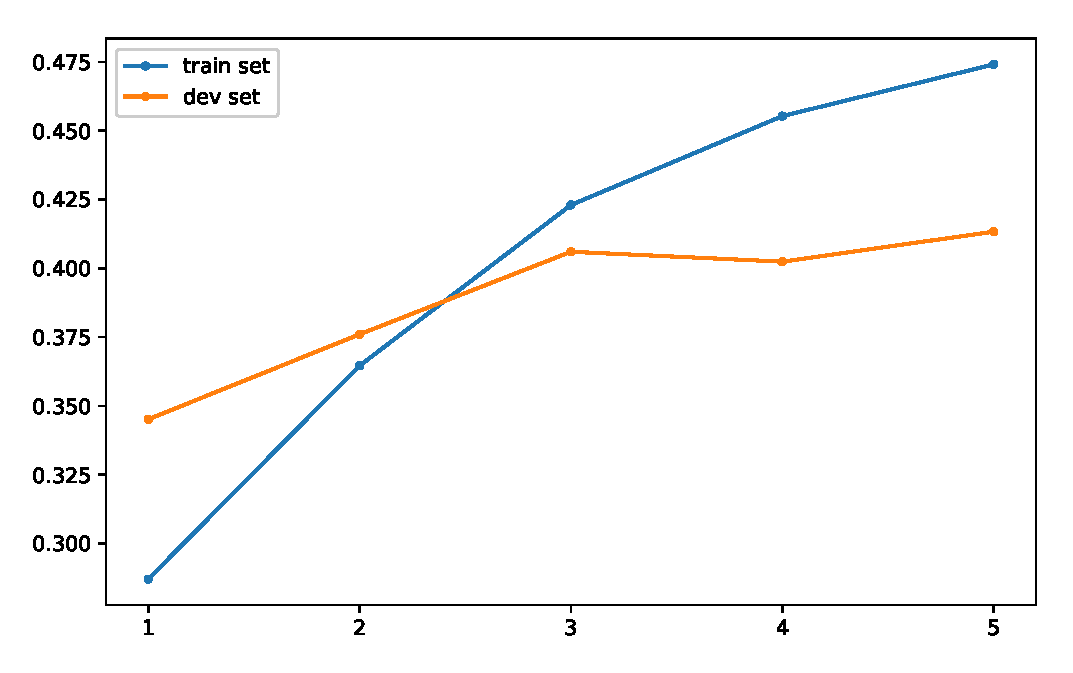
\includegraphics[scale=0.5]{plot.eps}  \\
\caption{Accuracies on the train and dev set}
\end{figure}

\begin{enumerate}[label=(\alph*)]
\setcounter{enumi}{2}
\item The architecture I experimented with is a 1D CNN followed by Maxpooling and a LSTM. Because of the Maxpooling it is much faster to train than the vanilla LSTM. Some dropout is added to prevent overfitting. For some runs it slightly outperformed the previous architecture.
\end{enumerate}
\end{document}